%!TEX program = xelatex
\documentclass[12pt, a4paper, fontset=none]{ctexart}
\usepackage{geometry}
\usepackage{booktabs}
\usepackage{longtable}
\usepackage{array}
\usepackage{amsmath}
\usepackage{graphicx}
\usepackage{float}
\usepackage{hyperref}
\geometry{left=2.5cm, right=2.5cm, top=2.5cm, bottom=2.5cm}
\setCJKmainfont{Songti SC}
\setCJKsansfont{Heiti SC}
\setCJKmonofont{STSong}

\title{\textbf{岗位综合化趋势：Global LDA 与 LDA Alignment 双方法对比报告}}
\date{2026年2月8日}

\begin{document}
\maketitle

% ============================================================
\section{研究问题}
% ============================================================

近年来，一个直觉上的观察是：随着AI工具的普及，许多岗位的职责范围似乎在变宽——一个人可能需要同时承担过去由多个人分工完成的任务。我们把这种现象称为\textbf{岗位综合化}。

但"综合化"是一个模糊的概念。要把它变成可以量化、可以跨年比较的指标，我们需要回答三个子问题：

\begin{enumerate}
    \item 如何从招聘广告的文本中提取出"这个岗位涉及哪些技能领域"？
    \item 如何把“任务或职能的多样性”变成一个数字？
    \item 这个数字在2016--2025年间是否呈上升趋势？
\end{enumerate}

我们在此用两套独立方法回答上述问题，并对比两者的结论是否一致。

% ============================================================
\section{从文本到"技能配方"：LDA主题模型}
% ============================================================

\subsection{文献综述：LDA 研究进展与本文切入点}

围绕“如何刻画岗位技能综合化及其时序演化”这一问题，现有 LDA 研究在总体上形成了清晰而连续的知识链条。首先，Blei, Ng, \& Jordan (2003) 建立了“文档--主题分布”与“主题--词分布”的基础概率框架，为后续研究提供了共同起点。其次，在这一框架基础上，Zhu et al. (2016)、Han (2020) 与 Liu et al. (2020) 将研究重心推进到时间维度，持续讨论主题的演化、漂移与路径映射。与此同时，Malik et al. (2013) 从可视化对齐角度增强了跨时段解释能力，而 Yang et al. (2024) 与 Palamarchuk et al. (2025) 分别从 coherence 引导与 temporal embeddings 可视分析出发，进一步提升了主题模型的可解释性与可操作性。然而，上述路径也显示出一个共同张力：在强化跨年可比性的同时，往往会降低对结构突变的敏感性；反之，强调局部演化识别时，又可能牺牲全局可比性。

总体上，已有研究已经回答了“能否识别主题、能否追踪变化、能否提升解释性”；但在大规模岗位文本场景中，仍需进一步回答：\textbf{如何同时度量综合化程度（量）与结构重组路径（形）}。这正是本文的学术对话点与研究切入点。

具体地，本文采用“统一主题空间 LDA（方法一）+ Window LDA Alignment（方法二）”的双方法路径：前者强调跨期可比，后者强调演化识别，二者互补验证。

形式上，对于任一招聘广告 \(d\)，LDA 输出长度为 \(K\) 的主题概率向量：
\[
    \boldsymbol{\theta}_d = (p_1, p_2, \ldots, p_K), \quad \text{其中 } p_k \geq 0 \text{ 且 } \sum_{k=1}^{K} p_k = 1
\]
其中 \(p_k\) 表示岗位在第 \(k\) 个主题上的权重（关联强度）。

\subsection{统一主题空间 LDA（方法一）}

方法一采用的是\textbf{统一主题空间 LDA 策略}（global-topic-space LDA strategy）：在2016--2025年全部招聘广告上训练一个统一的50主题模型，而不是按年份分别训练。其直接优势是跨年可比性强，即2016年的“主题3”和2024年的“主题3”处于同一语义坐标系，可解释为同一技能领域。

在本研究中，该策略主要用于回答“岗位综合化程度是否上升”这一问题，后续的 Entropy/HHI 年度趋势均基于该统一主题空间计算得到。

\subsection{Window LDA + Alignment（方法二）}

与统一主题空间 LDA 不同，方法二采用\textbf{分窗口建模}：先在各时间窗口内独立训练 LDA，再对相邻窗口的主题进行对齐，用于识别结构演化路径（存活/分裂/融合）。

\textbf{本项目中实际采用的对齐流程如下：}
\begin{enumerate}
    \item 对每个窗口独立训练 LDA，并将窗口内主题向量化（用于跨窗口比较）。
    \item 对相邻窗口 \(t\) 与 \(t+1\) 构建主题余弦相似度矩阵 \(S\)。
    \item 在 \(S\) 上先用匈牙利算法做一对一最优匹配，将相似度高于阈值（代码中为 0.7）的匹配记为 \textbf{Survival}。
    \item 对未匹配主题再做阈值贪婪搜索（代码中阈值为 0.5）：识别“多对一”的 \textbf{Merge} 与“一对多”的 \textbf{Split}。
    \item 输出窗口级指标（Survival率、Split率、Merge率）与事件明细表，用于比较不同时段的结构重组强度。
\end{enumerate}

\textbf{方法参考文献（APA）：}
\begin{itemize}
    \item Blei, D. M., Ng, A. Y., \& Jordan, M. I. (2003). Latent Dirichlet allocation. \textit{Journal of Machine Learning Research, 3}, 993--1022. \url{https://jmlr.org/papers/v3/blei03a.html}
    \item Han, X. (2020). Evolution of research topics in LIS between 1996 and 2019: An analysis based on latent Dirichlet allocation topic model. \textit{Scientometrics, 125}(3), 2561--2595. \url{https://doi.org/10.1007/s11192-020-03721-0}
    \item Liu, H., Chen, Z., Tang, J., Zhou, Y., \& Liu, S. (2020). Mapping the technology evolution path: A novel model for dynamic topic detection and tracking. \textit{Scientometrics, 125}(3), 2043--2090. \url{https://doi.org/10.1007/s11192-020-03700-5}
    \item Malik, S., Smith, A., Hawes, T., Papadatos, P., Li, J., Dunne, C., \& Shneiderman, B. (2013). TopicFlow: Visualizing topic alignment of Twitter data over time. In \textit{Proceedings of the 2013 IEEE/ACM International Conference on Advances in Social Networks Analysis and Mining} (pp. 720--726). Association for Computing Machinery. \url{https://doi.org/10.1145/2492517.2492639}
    \item Palamarchuk, D., et al. (2025). Visualizing temporal topic embeddings with a compass. \textit{IEEE Transactions on Visualization and Computer Graphics, 31}(1), 272--282. \url{https://doi.org/10.1109/TVCG.2024.3456143}
    \item Yang, H., Li, J., \& Chen, S. (2024). TopicRefiner: Coherence-guided steerable LDA for visual topic enhancement. \textit{IEEE Transactions on Visualization and Computer Graphics, 30}(8), 4542--4557. \url{https://doi.org/10.1109/TVCG.2023.3266890}
    \item Zhu, C., Zhu, H., Ge, Y., Chen, E., Liu, Q., Xu, T., \& Xiong, H. (2016). Tracking the evolution of social emotions with topic models. \textit{Knowledge and Information Systems, 47}(3), 517--544. \url{https://doi.org/10.1007/s10115-015-0865-0}
\end{itemize}

% ============================================================
\section{如何量化描述综合化程度}
% ============================================================

有了每条招聘广告的技能配方$(p_1, p_2, \ldots, p_K)$之后，下一个问题是：怎么衡量这份配方到底有多"综合"？

举一个直观的对比：
\begin{itemize}
    \item 一个纯粹的Java程序员岗位，也许90\%的权重集中在"软件开发"这一个主题上——这是\textbf{专业化}。
    \item 一个创业公司的产品经理，可能30\%编程、25\%数据分析、25\%沟通协调、20\%项目管理——这是\textbf{综合化}。
\end{itemize}

我们需要一个数字来区分这两种情况。这里借用了两个有坚实理论基础的经典指标。

\subsection{指标一：主题熵（Normalized Shannon Entropy）}

Shannon熵源自信息论，衡量一个概率分布的"不确定性"或"分散程度"：

\[
    H(d) = -\frac{\sum_{k=1}^{K} p_k \ln p_k}{\ln K}
\]

分母$\ln K$是一个标准化系数（$K$个主题均匀分布时的最大熵值），使$H$的取值范围恰好为$[0, 1]$：

\begin{itemize}
    \item $H = 0$：所有概率集中在一个主题上。这个岗位是极端的"专才"——只涉及一种技能。
    \item $H = 1$：概率在50个主题上完全均匀分布。这个岗位是极端的"通才"——均匀涉及所有技能。
    \item 现实中的岗位介于两者之间，$H$越大表示越综合。
\end{itemize}

\textbf{为什么用它？} 熵对分布的尾部比较敏感——即使一个岗位在很多冷门主题上只有很小的概率（比如5\%的法律、3\%的设计），熵也会捕捉到这种"涉猎广泛但每项不深"的综合化特征。

\subsection{指标二：HHI 集中度指数（Herfindahl-Hirschman Index）}

HHI是经济学中衡量市场集中度的经典工具。在反垄断分析中，如果少数企业占据了大部分市场份额，HHI就高，意味着市场被少数巨头垄断。我们把同样的逻辑移植到岗位技能上——把"企业的市场份额"替换为"技能主题的权重占比"：

\[
    \text{HHI}(d) = \sum_{k=1}^{K} p_k^2
\]

\begin{itemize}
    \item $\text{HHI} = 1$：所有权重集中在一个主题上（极端专业化，如同一家企业占据整个市场）。
    \item $\text{HHI} = 1/K = 0.02$：完全均匀分布（极端综合化，如同50家企业各占2\%市场份额）。
    \item HHI越低，技能分布越分散，岗位越综合。
\end{itemize}

\textbf{为什么用它？} 与熵相反，HHI对分布的头部更敏感——它主要由权重最大的那几个主题决定。如果一个岗位从"一个主题占80\%"变成"两个主题各占40\%"，HHI会有明显下降。

\subsection{为什么同时用两个指标？}

\begin{table}[h]
\centering
\caption{两个指标的互补性}
\begin{tabular}{lcc}
\toprule
& \textbf{Entropy（熵）} & \textbf{HHI} \\
\midrule
学科来源 & 信息论 & 产业经济学 \\
敏感区域 & 尾部（小权重主题） & 头部（大权重主题） \\
方向 & 越高越综合 & 越低越综合 \\
\bottomrule
\end{tabular}
\end{table}

如果两个指标的年度趋势方向一致（熵上升且HHI下降），我们对"综合化确实在发生"的结论就更有信心——因为它不是某个特定指标的计算伪影，而是两种不同视角下共同观察到的现象。

% ============================================================
\section{Global LDA 结果}
% ============================================================

我们对776万条招聘广告（2016--2025年）逐条计算了上述两个指标，然后按年取平均值。

\begin{figure}[h]
\centering
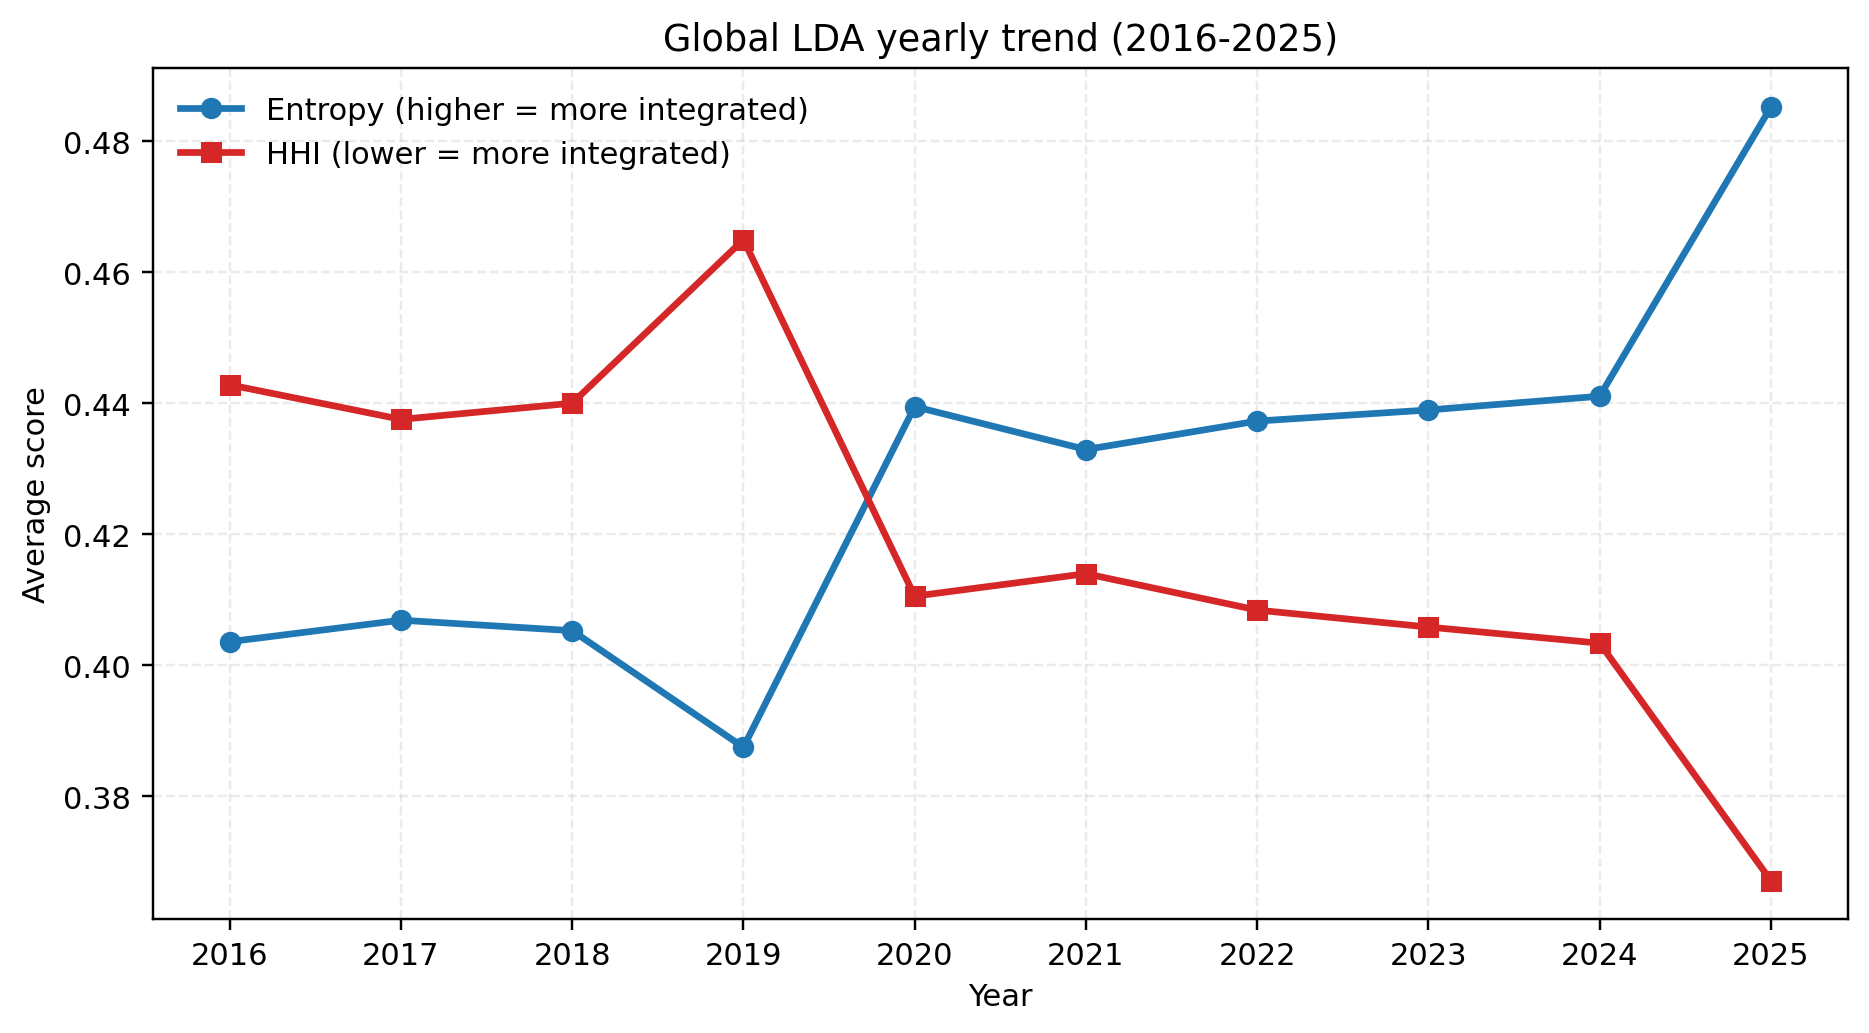
\includegraphics[width=0.88\textwidth]{figures/global_lda_yearly_trend.png}
\caption{Global LDA 年度趋势折线图（2016--2025）}
\label{fig:global_lda_yearly_trend}
\end{figure}

\begin{longtable}{cccc}
\caption{Global LDA 年度统计}\\
\toprule
年份 & 样本量 $N$ & 平均 Entropy $\overline{H}$ & 平均 HHI \\
\midrule
\endfirsthead
\toprule
年份 & 样本量 $N$ & 平均 Entropy $\overline{H}$ & 平均 HHI \\
\midrule
\endhead
2016 & 486,319 & 0.4036 & 0.4428 \\
2017 & 871,057 & 0.4069 & 0.4375 \\
2018 & 417,985 & 0.4053 & 0.4400 \\
\midrule
\multicolumn{4}{c}{\textit{2019--2020年数据严重缺失（2019仅13条），趋势断裂}} \\
\midrule
2021 & 1,235,457 & 0.4329 & 0.4140 \\
2022 & 2,321,292 & 0.4373 & 0.4084 \\
2023 & 1,241,792 & 0.4390 & 0.4058 \\
2024 & 1,172,035 & 0.4411 & 0.4034 \\
2025 & 21,203$^*$ & 0.4852 & 0.3671 \\
\bottomrule
\multicolumn{4}{l}{\footnotesize $^*$ 2025年为不完整年份，样本量仅为2024年的1.8\%，需谨慎解读。}
\end{longtable}

\subsection{趋势解读}

两个指标讲述了同一个故事：

\begin{itemize}
    \item \textbf{2016--2018年（AI应用渗透早期）}：Entropy稳定在0.404附近，HHI稳定在0.440附近。岗位的技能综合化程度基本没有变化，说明这一阶段AI对岗位结构的改写仍较有限。
    \item \textbf{2018 $\rightarrow$ 2021年（AI应用加速扩散期）}：Entropy从0.405跳升至0.433（+6.9\%），HHI同步下降。这是样本期内最大的一次跳变，表明岗位技能组合开始明显由单一职能向复合职能迁移。
    \item \textbf{2021--2024年（生成式AI扩散期）}：Entropy从0.433缓慢上行至0.441（+1.9\%），趋势平稳持续。尽管ChatGPT于2022年11月发布，但2022--2024年的变化表现为渐进抬升而非一次性突变，反映出生成式AI影响通过组织采用与岗位重构逐步释放。
\end{itemize}

% ============================================================
\section{Alignment方法：另一个视角}
% ============================================================

Global LDA回答的是"综合化的\textbf{程度}有多大"。而Alignment方法回答的是另一个问题："JD中涉及的技能是如何演变的？"

\subsection{方法简介}

Alignment不使用全局模型，而是在每个两年窗口内独立训练LDA，得到各自的50个主题。然后，通过向量相似度将相邻窗口的主题一一对齐，识别三种演化事件：

\begin{itemize}
    \item \textbf{存活（Survival）}：窗口A的某个主题在窗口B中找到了高度相似的对应主题。说明该技能领域保持稳定，比如"财务会计"在前后两个时期都是独立且相似的主题。
    \item \textbf{分裂（Split）}：窗口A的一个主题在窗口B中对应了两个或更多新主题。说明该技能领域内部发生了分化——比如原来的"数据分析"分裂为"传统BI分析"和"AI/机器学习"两个方向。
    \item \textbf{融合（Merge）}：窗口A的两个主题在窗口B中合并为一个。说明原本独立的技能领域开始交叉——比如"市场营销"和"数据分析"合并为"数据驱动营销"。
\end{itemize}

\subsection{分窗口结果}

\begin{table}[h]
\centering
\caption{相邻窗口的结构演化对比}
\begin{tabular}{lcccc}
\toprule
\textbf{窗口对} & \textbf{存活率} & \textbf{分裂率} & \textbf{融合率} & \textbf{存活相似度} \\
\midrule
2016-2017 $\rightarrow$ 2018-2019 & 90.0\% & 7.5\% & 2.5\% & 0.913 \\
2018-2019 $\rightarrow$ 2020-2021 & 83.8\% & 8.1\% & 8.1\% & 0.916 \\
2020-2021 $\rightarrow$ 2022-2023 & 87.5\% & 5.0\% & 7.5\% & 0.895 \\
2022-2023 $\rightarrow$ 2024-2025 & 73.2\% & 12.2\% & 14.6\% & 0.909 \\
\bottomrule
\end{tabular}
\end{table}

\begin{figure}[h]
\centering
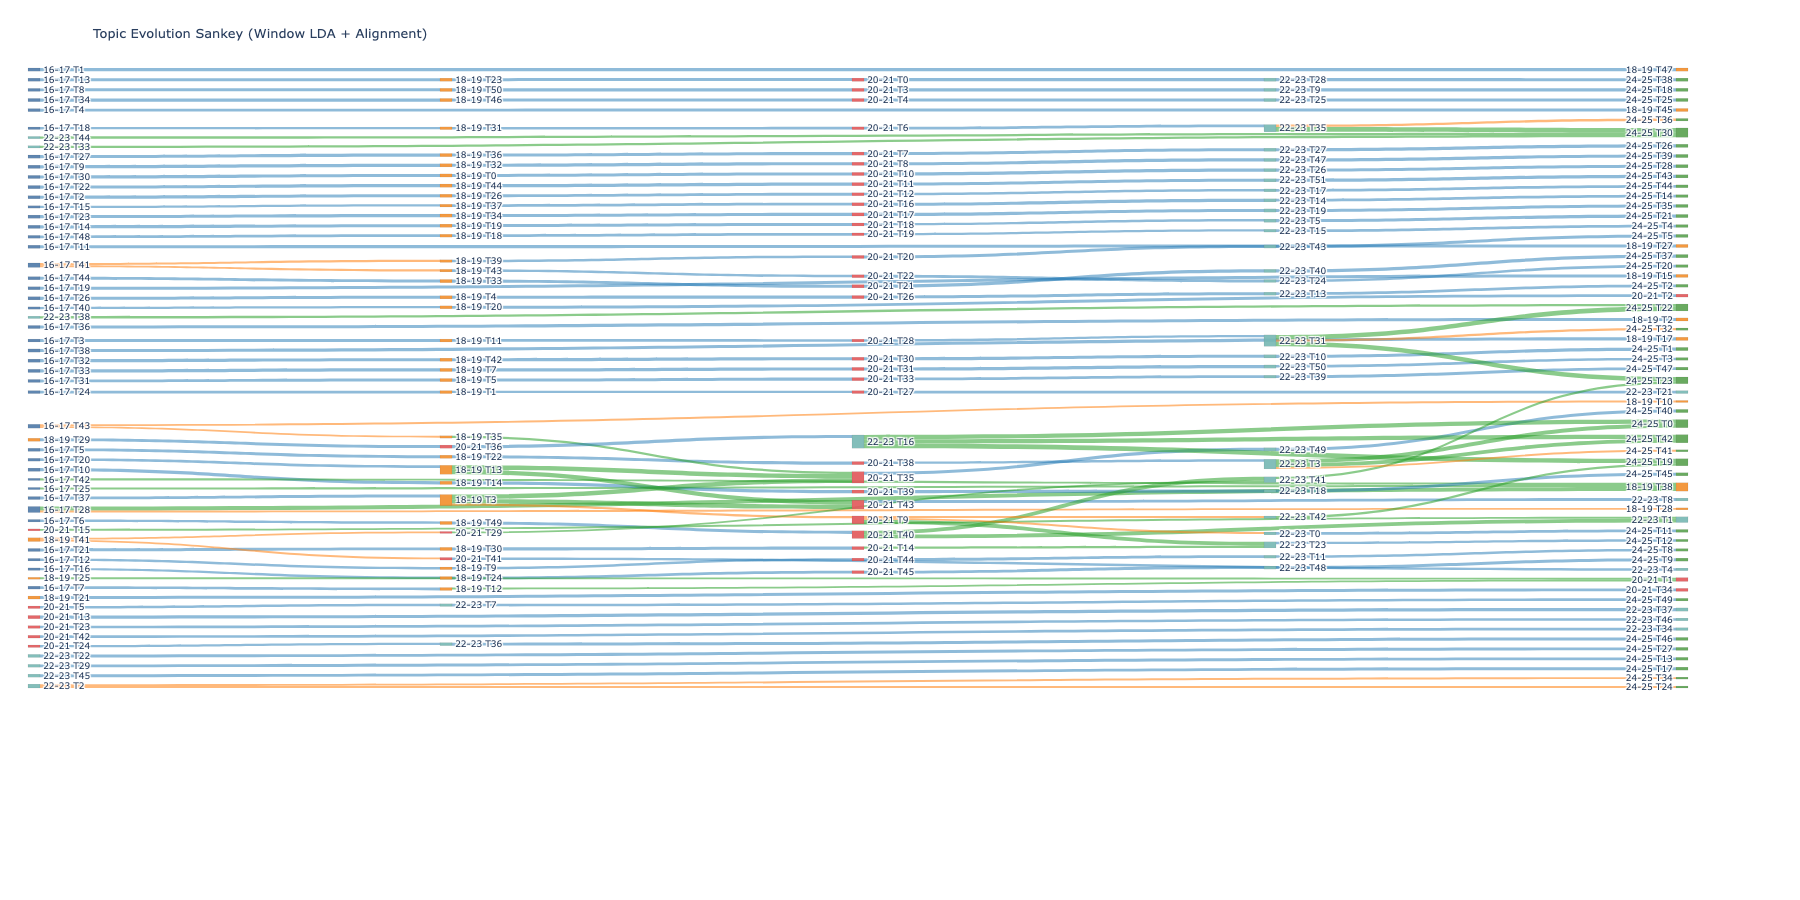
\includegraphics[width=0.98\textwidth]{figures/topic_evolution_sankey.png}
\caption{主题演化桑基图（Window LDA + Alignment）}
\label{fig:topic_evolution_sankey}
\end{figure}

\subsection{解读}

最引人注目的是最后一行：2022-2023 $\rightarrow$ 2024-2025窗口的存活率骤降至73.2\%，分裂率和融合率同时飙升。这意味着\textbf{超过四分之一}的技能领域在最近两年发生了结构性重组——有的领域一分为二（分化），有的领域合并交叉（融合）。

这与Global LDA的发现互相印证：综合化不仅体现为entropy的渐进上升（量变），也体现为技能领域边界的加速重组（质变）。

\subsubsection{比较有意思的合并与分裂技能丛}

结合图\ref{fig:topic_evolution_sankey}与事件明细，我们在最新窗口（2022-2023 $\rightarrow$ 2024-2025）中按相似度与主题可解释性筛选了三组代表性技能丛：

\begin{table}[H]
\centering
\caption{代表性合并/分裂技能丛（2022--2025）}
\begin{tabular}{p{0.13\textwidth}p{0.46\textwidth}p{0.30\textwidth}}
\toprule
\textbf{类型} & \textbf{技能丛演化（主题关键词）} & \textbf{含义} \\
\midrule
融合 & 责任心/协作（T31） + 采购/物流/供应链（T38） $\Rightarrow$ 产品/技术/研发（T22），$sim=0.720$ & 软技能与供应链执行能力向“产品技术化”任务汇聚。 \\
分裂 & 责任心/协作（T31） $\Rightarrow$ 产品研发（T22） + 检测检验（T23） + 市场管理（T32），$sim=0.702$ & 通用能力由“通识要求”分化为研发、质检、市场三条更专业路径。 \\
分裂 & 人力资源/数据分析（T3） $\Rightarrow$ 计划目标制定（T41） + 电气机电系统（T42） + 分析撰写（T0），$sim=0.603$ & HR-数据主题出现跨域迁移，反映职能边界重组与岗位复合化。 \\
\bottomrule
\end{tabular}
\end{table}

\subsubsection{长期存活的技能丛（跨 2016--2025 连续存活）}

除“合并/分裂”外，alignment 结果还显示出一批长期稳定存在的能力簇。基于四次连续 Survival 映射（2016-2017 $\rightarrow$ 2018-2019 $\rightarrow$ 2020-2021 $\rightarrow$ 2022-2023 $\rightarrow$ 2024-2025），可识别出以下代表性长期存活技能丛：

\begin{longtable}{p{0.45\textwidth}p{0.23\textwidth}p{0.22\textwidth}}
\caption{长期存活技能丛（连续四次 Survival）}\\
\toprule
\textbf{技能丛链条（merged topic labels）} & \textbf{平均相似度} & \textbf{解释} \\
\midrule
\endfirsthead
\toprule
\textbf{技能丛链条（merged topic labels）} & \textbf{平均相似度} & \textbf{解释} \\
\midrule
\endhead
熟练/办公软件/操作 $\rightarrow$ 熟练/办公软件/操作 $\rightarrow$ 熟练/办公软件/操作 $\rightarrow$ 熟练/办公软件/操作 $\rightarrow$ 熟练/办公软件/操作 & 0.986 & 通用数字办公能力长期稳定，是多数岗位的基础能力底座。 \\
设备/维修/安全 $\rightarrow$ 设备/维修/安装 $\rightarrow$ 设备/维修/维护 $\rightarrow$ 设备/维修/维护 $\rightarrow$ 设备/维修/操作 & 0.983 & 设备运维与维修类技能跨周期持续存在，体现实体运营岗位的稳定需求。 \\
销售/市场营销/行业 $\rightarrow$ 销售/行业/沟通 $\rightarrow$ 销售/市场/行业 $\rightarrow$ 销售/行业/市场营销 $\rightarrow$ 销售/行业/市场 & 0.975 & 销售与市场能力持续存活，并向更精细化市场运营演进。 \\
工程/施工/建筑 $\rightarrow$ 工程/施工/管理 $\rightarrow$ 工程/施工/管理 $\rightarrow$ 工程/施工/管理 $\rightarrow$ 工程/施工/管理 & 0.972 & 工程施工管理链条在全时段保持高稳定性，属于长期核心能力簇。 \\
教学/学生/教育 $\rightarrow$ 教育/培训/教学 $\rightarrow$ 教育/教学/学生 $\rightarrow$ 教育/教学/学生 $\rightarrow$ 教育/教学/培训 & 0.960 & 教育教学类能力跨阶段延续，显示该职业域的结构惯性较强。 \\
\bottomrule
\end{longtable}

\noindent 需要说明的是，2025年样本量较小，且少数主题存在文本噪声（如模板词），因此上述技能丛更适合作为“结构变化信号”而非一一对应的职业分类结论。

% ============================================================
\section{两套方法的并列比较}
% ============================================================

\begin{table}[h]
\centering
\caption{Global LDA（程度）与 Alignment（结构）的窗口级对比}
\begin{tabular}{p{0.24\textwidth}cccc}
\toprule
\textbf{窗口迁移} & \textbf{$\Delta$Entropy} & \textbf{$\Delta$HHI} & \textbf{存活率} & \textbf{重组率} \\
\midrule
2016-17 $\rightarrow$ 2018-19 & $-$0.11\% & $+$0.13\% & 90.0\% & 10.0\% \\
2018-19 $\rightarrow$ 2020-21 & $+$6.83\% & $-$5.92\% & 83.8\% & 16.2\% \\
2020-21 $\rightarrow$ 2022-23 & $+$1.14\% & $-$1.56\% & 87.5\% & 12.5\% \\
2022-23 $\rightarrow$ 2024-25 & $+$0.91\% & $-$1.18\% & 73.2\% & 26.8\% \\
\bottomrule
\end{tabular}
\end{table}

\noindent 这张表可以从左右两半分别阅读：
\begin{itemize}
    \item \textbf{左半部分}（$\Delta$Entropy/$\Delta$HHI）：衡量"平均每个岗位的技能组合是否变得更分散"——这是\textbf{程度}上的变化。
    \item \textbf{右半部分}（存活率/重组率）：衡量"技能领域本身的边界是否在重新划分"——这是\textbf{结构}上的变化。
\end{itemize}

两套方法的结论一致：
\begin{enumerate}
    \item \textbf{2016--2018年（AI应用渗透早期）}：岗位技能结构基本稳定，综合化程度没有明显变化。
    \item \textbf{2018--2021年（AI应用扩散加速期）}：综合化程度显著跳升（$\Delta$Entropy +6.83\%），技能结构也开始松动（重组率16.2\%）。
    \item \textbf{2021--2025年（生成式AI扩散期）}：综合化程度继续缓慢推进，但最新窗口的结构重组明显加速（重组率26.8\%），说明技能领域边界正在被快速改写。
\end{enumerate}

% ============================================================
\section{关于2025年数据的说明}
% ============================================================

2025年的数据仅覆盖了部分月份（$N = 21{,}203$），远低于其他年份（$N > 40$万）。因此：

\begin{enumerate}
    \item \textbf{主结果}中保留2025年的数据点，但在图表中以不同符号或虚线标注其不完整性。
    \item \textbf{稳健性检验}中，额外提供"不含2025年"的趋势图，以确认主要结论不依赖于这一不完整年份。
\end{enumerate}

% ============================================================
\section{复现提示}
% ============================================================

\begin{itemize}
    \item Global LDA 推断结果文件：\texttt{output/final\_results\_sample.csv}
    \item Alignment 事件文件：\texttt{output/lda/alignment/topic\_evolution\_events.csv}
    \item Alignment 汇总对象：\texttt{output/lda/alignment/alignment\_results.pkl}
\end{itemize}

\end{document}
